%\documentclass[xcolor={dvipsnames}, handout]{beamer}
\documentclass[xcolor={dvipsnames}]{beamer}
%\usepackage{amsmath,amsfonts,amssymb,pxfonts,eulervm,xspace}
\usepackage{amsmath, amsfonts, amssymb, mathtools, eulervm, xspace}
\usepackage{bm}
\usepackage{mathrsfs} % math script fonts
\usepackage{tikz}

\usetikzlibrary{cd} % commutative diagrams
\usepackage{subcaption} % subfigure float captioning

\usepackage{tabulary}
\usepackage{multirow}
\usepackage{graphicx}

\usepackage{appendixnumberbeamer} 
\usepackage{minted}
\setminted[python]{fontsize=\scriptsize, 
                   linenos,
                   numbersep=8pt,
                   autogobble, 
                   frame=lines,
                   bgcolor=bg,
                   framesep=3mm} 
\usepackage{notation} % move this later

\graphicspath{.figures/}

\usepackage[backend=bibtex, style=numeric-comp, sorting=none, doi=false,isbn=false,url=false, giveninits=true]{biblatex}
\bibliography{../draft/glasslab_viz.bib}

\usetheme{ccnycrest}

\newenvironment{changemargin}[2]{%
\begin{list}{}{%
\setlength{\topsep}{0pt}%
\setlength{\leftmargin}{#1}%
\setlength{\rightmargin}{#2}%
\setlength{\listparindent}{\parindent}%
\setlength{\itemindent}{\parindent}%
\setleng{}th{\parsep}{\parskip}%
}%
\item[]}{\end{list}}

\begin{document}

\title{Topological Equivariant Artist Model}

\begin{frame}
	\titlepage
    Hannah Aizenman\\
    Advisor: Dr. Michael Grossberg \\
    Committee: Dr. Robert Haralick, Dr. Lev Manovich, Dr. Huy Vo\\
    External Member: Dr. Marcus Hanwell
\end{frame}

\section{Introduction}

\begin{frame}{Visualizations are structure preserving maps}
    \begin{figure}
        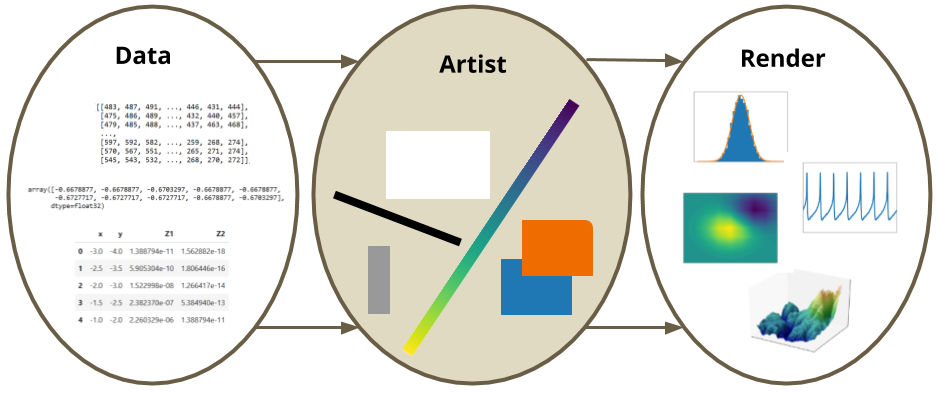
\includegraphics[width=1\linewidth]{figures/intro/dar.png}
    \end{figure}
    The aim of this work is to rearchitecture Matplotlib
    \pause 
    to take advantage of developments in software design, data structures, and visualization
    \pause
    to improve consistency, reusability, and discoverability,
    \pause
    so domain specific tool developers can build structure preserving visualization tools.
\end{frame}

\begin{frame}{Visualization component constraints}
    \begin{description}
        \item[equivariance] properties of data and visual encoding match
        \item[continuity] connectivity of data and visual encoding match
        \item[composibility] structure preserved by individual components is preserved in combined components
    \end{description}
\end{frame}

\subsection{Background}
\begin{frame}{Tools are tuned to date continuity \cite{HeerSoftware2006}}
    \begin{columns}
            \column{0.33\textwidth}
            \begin{figure}
                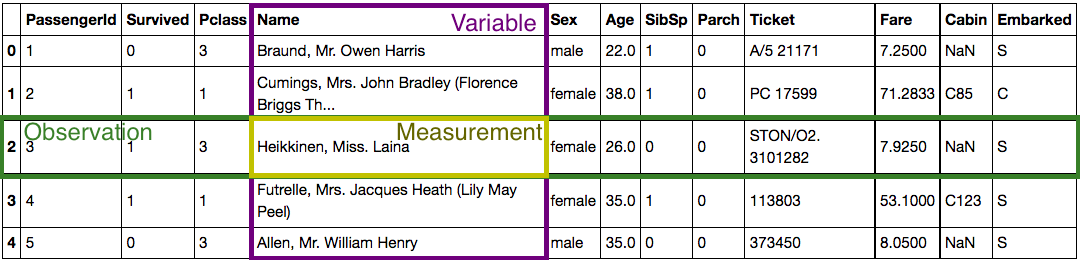
\includegraphics[width=1\textwidth]{figures/intro/data_formatting.png}
                \caption{Based on fig~2.5 in Munzner's VAD\cite{munznerVisualizationAnalysisDesign2014}}
            \end{figure}
            \begin{enumerate}
                \item Tableau\cite{StoltePolaris2002,hanrahanVizQL2006,MackinlayShowme2007}
                \item ggplot\cite{wickhamGgplot2ElegantGraphics2016a}
                \item Vega\cite{satyanarayanDeclarativeInteractionDesign2014}, Altair\cite{vanderplasAltairInteractiveStatistical2018}
            \end{enumerate}
            \pause
            \column{0.33\textwidth}
            \begin{figure}
                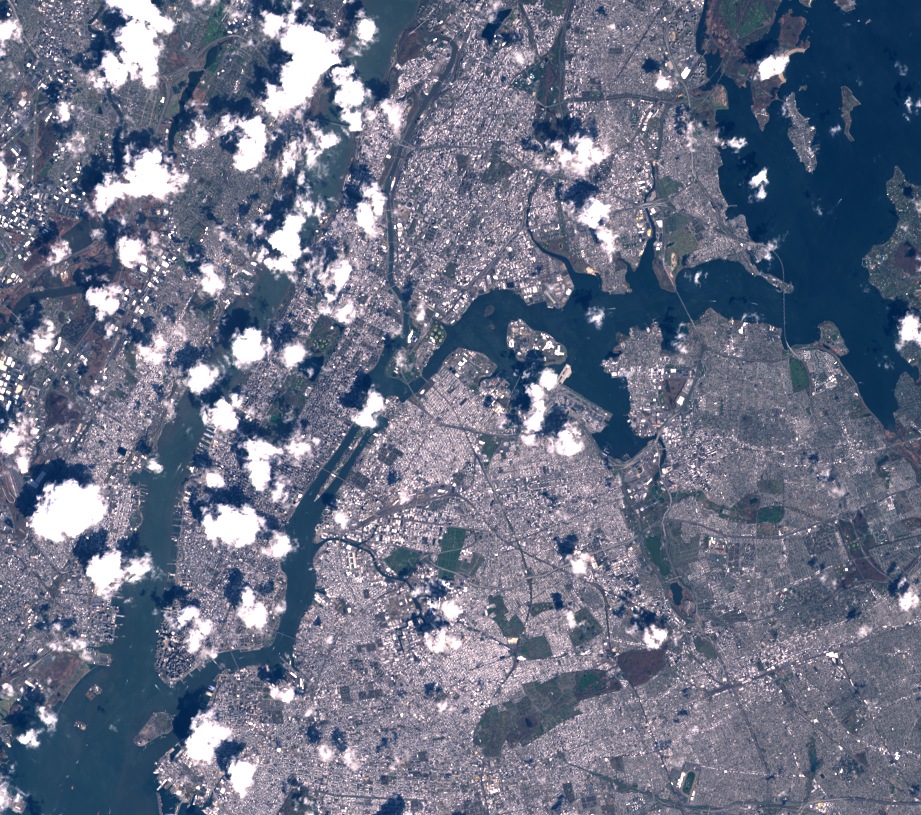
\includegraphics[width=1\textwidth]{figures/intro/landsat.png}
            \end{figure}
            \begin{enumerate}
                \item ImageJ\cite{schneiderNIHImageImageJ2012}, ImagePlot\cite{studiesCulturevisImageplot2021}
                \item Napari\cite{nicholas_sofroniew_2021_4533308}
            \end{enumerate}
            \pause
            \column{0.33\textwidth}
            \begin{figure}
                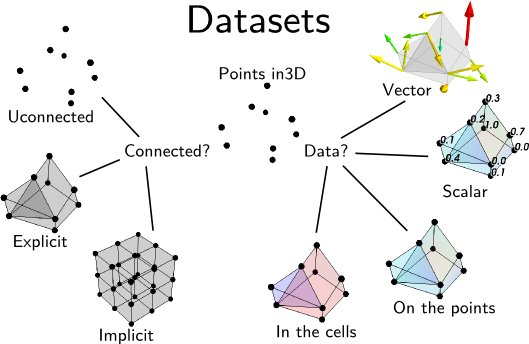
\includegraphics[width=1\textwidth]{figures/intro/dataset_diagram.png}
                \caption{Data Representation, MayaVi 4.7.2 docs\cite{DataRepresentationMayavi}}
            \end{figure}
            \begin{enumerate}
                \item Gephi\cite{bastianGephiOpenSource2009}
                \item Graphviz\cite{ellsonGraphvizOpenSource2002}
                \item Networkx\cite{HagbergExploringNetwork2008}
            \end{enumerate}
    \end{columns}
\end{frame}

\begin{frame}{Visualizations are tuned to data continuinity\cite{toryRethinkingVisualizationHighlevel2004}}
    \begin{figure}
        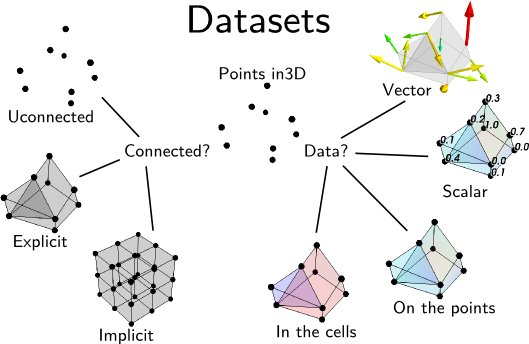
\includegraphics[height=.5\textheight]{figures/intro/dataset_diagram.png}
        \caption{Data Representation, MayaVi 4.7.2 docs\cite{DataRepresentationMayavi}}
    \end{figure}
    \begin{enumerate}
        \item Matplotlib\cite{hunterMatplotlib2DGraphics2007}, 
        \item D3 \cite{bostockDataDrivenDocuments2011}
        \item VTK \cite{hanwellVisualizationToolkitVTK2015,geveci2012vtk}, MayaVi\cite{RamachandranMayaVI2011}, ParaView\cite{ahrens2005paraview}, Titan\cite{brianwylieUnifiedToolkitInformation2009}
    \end{enumerate}
\end{frame}

\begin{frame}{Structure is encoded in variables and continuity}
    \begin{figure}
        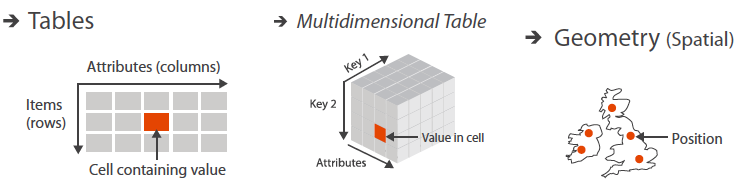
\includegraphics[width=1\textwidth]{figures/intro/munzner_datatypes.png}
        \caption{Image is figure 2.8 in Munzner's Visualization Analysis and Design\cite{munznerVisualizationAnalysisDesign2014}}
    \end{figure}
    \begin{description}
        \item[binding] metadata are structural \textit{keys} with associated \textit{values} (Munzner \cite{munznerVisualizationAnalysisDesign2014})] 
        \item[continuity] Fiber bundles can be a common data abstraction (Butler \cite{butlerVectorBundleClassesForm1992,butlerVisualizationModelBased1989})
        \item[variables] Fibers can hold schema like encodings of variables (Spivak \cite{spivakDatabasesAreCategories2010,spivakSIMPLICIALDATABASES})
    \end{description}
\end{frame}

\begin{frame}{Visualizations are (mostly) evaluated on equivariance}
    \begin{description}
        \item[Expressiveness] structure preserving mappings from data to graphic (Mackinlay \cite{mackinlayAutomatingDesignGraphical1986})
        \item[Effectiveness] design choices made in deference to perceptual saliency (Mackinlay \cite{clevelandResearchStatisticalGraphics1987,clevelandGraphicalPerceptionTheory1984,chambersGraphicalMethodsData1983a, munznerVisualizationAnalysisDesign2014})
        \item[Naturalness] easier to understand when properties match (Norman \cite{norman_things_smart})
        \item[Graphical Integrity] graphs show \textbf{only} the data (Tufte \cite{tufteVisualDisplayQuantitative2001})
    \end{description}
\end{frame}


\begin{frame}{Models describe composition}
    \begin{description}
        \item[language model] APT, GoG: syntax, semantics, and grammar of graphics (Mackinlay, Wilkenson  \cite{mackinlayAutomatingDesignGraphical1986, mackinlayAUTOMATICDESIGNGRAPHICAL1987,wilkinsonGrammarGraphics2005})
        \item[functional dependencies] constrained maps between data and visual representation(Sugibuchi \cite{sugibuchiFramwork2009}) 
        \item[category theory] the semiotics of visualization are commutative (Vickers \cite{vickersUnderstandingViz2013})
        \item[algebraic process] data ($\alpha$) and viz ($\omega$) transforms are symmetric (Kindlmann and Scheidegger \cite{kindlmannAlgebraicProcessVisualization2014})
        \begin{columns}
            \column{.5\textwidth}
       
            \begin{description}
                \item[D] data 
                \item[R] representations
                \item[V] visualizations
            \end{description}
            \column{.5\textwidth}
            \begin{equation*}
                \begin{tikzcd}[ampersand replacement=\&]
                    D \arrow[d, "\alpha"'] \arrow[r, "r_1"] \& R \arrow[r, "\nu"]  \& V \arrow[d, "\omega"] \\
                    D \arrow[r, "r_2"']                     \& R \arrow[r, "\nu"'] \& V                    
                \end{tikzcd}
                \end{equation*}
       
        \end{columns} 
     
    \end{description}
\end{frame}


\subsection{Contributions}
\begin{frame}{Contributions}
    \begin{description}
        \item[Topological] topology preserving relationship between data and graphic via continuous maps
        \item[Equivariant] property preservation from data component to visual representation as equivariant maps that carry a homomorphism of monoid actions
        \item[Artist] functional oriented visualization tool architecture built on the mathematical model to demonstrate the utility of the model
        \item [Model] prototype of the architecture built on Matplotlib's infrastructure to demonstrate the feasibility of the model
    \end{description}
\end{frame}

\section{Mathematical Framework}

\begin{frame}{Topological Equivariant Artist Model}
    The Artist $\mathscr{\vartist}$ is a map from data $\mathscr{\dtotal}$ to graphic $\mathscr{\gtotal}$
    \begin{equation}
        \mathscr{\vartist}: \mathscr{\dtotal} \rightarrow \mathscr{\gtotal}
    \end{equation}
    \pause
     that carries a homomorphism of monoid actions 
    \begin{equation}
    \varphi: \monoid \rightarrow \monoid^{\prime}
    \end{equation}
    \pause
    such that artists are equivariant maps 
    \begin{equation}
    \mathscr{\vartist}(m\cdot \delement) = \varphi(m)\cdot\mathscr{\vartist}(\delement) 
    \end{equation}
    \pause 
    with a deformation retraction from graphic to data space. 
    \note{some kinda words about the continuity}
\end{frame}

\subsection{Data Model}

\begin{frame}{Data Bundle}
    \begin{figure}
        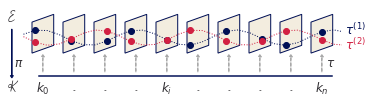
\includegraphics[width=1\textwidth]{figures/math/fiberbundle.png}
    \end{figure}
    A fiber bundle is a tuple $(\dtotal,\,\dbase,\,\pi ,\,\dfiber)$ defined by the projection map $\pi$
    \begin{equation}
        \label{eq:fiber_bundle}
        \begin{tikzcd}[ampersand replacement=\&]
            \dfiber \arrow[r, hook] \& \dtotal \arrow[r, "\pi"] \& \dbase
        \end{tikzcd}
    \end{equation}
    where \dtotal\ is the total data space, \dfiber\ is the variable space, and \dbase\ encodes the continuity.
\end{frame}

\begin{frame}{Variables: Fiber}
    Given a space of all possible values \ftotal\
    \begin{equation}
        \label{eq:data_types}
        \begin{tikzcd}[ampersand replacement=\&]
            \fttype \arrow[r] \arrow[d, "\pi_{\fsection}"'] \& \ftotal \arrow[d, "\pi"] \\
            \fnames \arrow[r, "\fsection"']                  \& \ftypes       
        \end{tikzcd}
    \end{equation}
    a fiber component is the restricted space $\ftotal_{\fsection(\fname)}$. 
    \begin{equation}
        \dfiber = \ftotal_{\fsection(\fname)} = \ftotal_{\ftype} 
    \end{equation}
    \begin{description}
        \item[\ftypes] data types of the variables in the dataset 
        \item[\ftotal] disjoint union of all values of type $\ftype \in \ftypes$ 
        \item[\fnames] variable names, $\fname \in \fnames$
        \item[\fttype] \ftotal\ restricted to the data type of a named variable   
    \end{description}
\end{frame}

\begin{frame}{Variable types are dimensions of the fiber}
    \begin{figure}[H]
        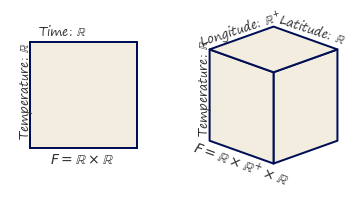
\includegraphics[width=\textwidth]{figures/math/fiber.png}
        \caption{}
        \label{fig:data_fiber_example}
    \end{figure}
    \begin{description}
        \item[plane]  $\dfiber=\reals\times\reals$, (time, temperature)
        \item[cube]  $\reals\times\realsp\times\reals$, (time, wind=(speed, direction))
    \end{description}
\end{frame}


\begin{frame}{Structure of Components: Monoid \& Monoid Actions}
A monoid \monoid\ is a set with
\begin{description}
    \item[associative binary operator] $\ast:\monoid \times \monoid\rightarrow \monoid$
    \item[identity element] $e\in \monoid$ such that $e\ast a= a \ast e = a$ for all $a \in \monoid$. 
\end{description}
\pause
\begin{block}{left monoid action}
A set \dfiber\ with an action\cite{nlab:action} $\bullet: \monoid\times \dfiber \rightarrow \dfiber$ with the properties:
    \begin{align*}
        \textbf{associativity}\;& \text{for all } f,g \in \monoid \text{ and } x\in \dfiber,\, f\bullet(g\bullet x) = (f\ast g) \bullet x\\
        \textbf{identity}\;& \text{for all } x\in \dfiber, e\in \monoid,\,  e\bullet x = x 
    \end{align*}
\end{block}
\end{frame}

\begin{frame}{Monoid Actions: Permutation}
    \begin{figure}
        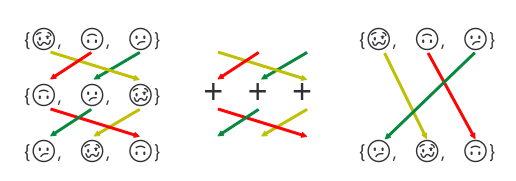
\includegraphics[width=1\linewidth]{figures/math/monoid_emoji.png}
    \end{figure}
\end{frame}

\begin{frame}{Why monoids? partial orders}
    \begin{figure}
        \begin{overprint}
            \onslide<1|handout:0>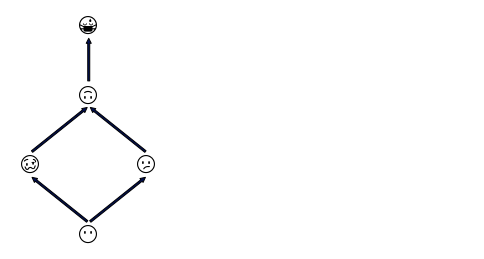
\includegraphics[width=1\linewidth]{figures/math/monoid_hasse.png}
            \onslide<2|handout:0>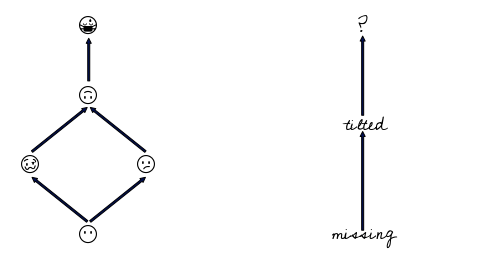
\includegraphics[width=1\linewidth]{figures/math/monoid_monotone.png}
            \onslide<3>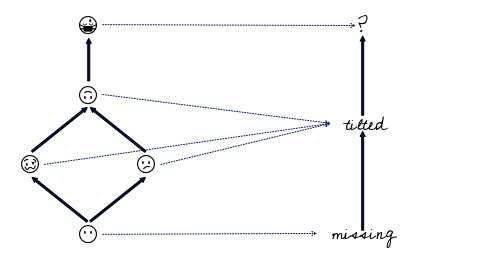
\includegraphics[width=1\linewidth]{figures/math/monoid_maps.png}
        \end{overprint}
    \caption{Inspired by definition 1.59 diagram in Spivak and Fong's An Invitation to Applied Category Theory \cite{fongInvitationAppliedCategory2019}}
    \end{figure}
\end{frame}

\begin{frame}{Data Continuity: Base space}
    \begin{figure}[H]
    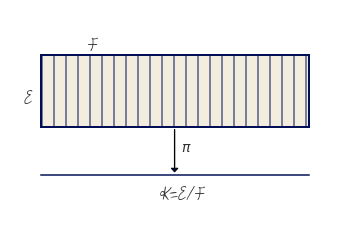
\includegraphics[height=.5\textheight]{figures/math/k_qspace.png}
    \label{fig:base_space_div}
\end{figure}
where the total space can be decomposed into components 
\begin{equation}
    \pi:\dtotal_1\oplus\ldots\oplus \dtotal_i \oplus\ldots \oplus \dtotal_n \rightarrow \dbase
\end{equation}
\end{frame}

\begin{frame}{Data connectivity is encoded as the base space}
    \begin{figure}[H]
        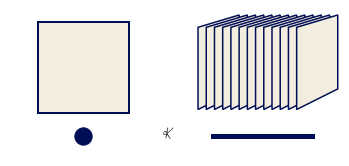
\includegraphics[width=1\textwidth]{figures/math/base.png}
        \caption{}
        \label{fig:base_example}
    \end{figure}
    \begin{description}
        \item[points] data is 0D discrete
        \item[line]  data is lies on the 1D continuous interval \dbase\
    \end{description}
\end{frame}

\begin{frame}{Values: Section}
    For any fiber bundle, there exists a map
    \begin{equation}
        \begin{tikzcd}[ampersand replacement=\&]
            \dfiber \arrow[r, hook] \& \dtotal \arrow[d, "\pi"'] \\
                              \& \dbase \arrow[u, "\dsection"', bend right]
        \end{tikzcd}
    \end{equation}
     s.t. $\pi(\dsection(\dbasepoint)) = \dbasepoint$.  Set of all global sections is denoted $\Gamma(\dtotal)$.
     \pause
     \begin{block}{Record}
     Assuming a trivial fiber bundle $\dtotal = \dbase \times \dfiber$, the section is 
\begin{equation}
    \label{eq:section_return}
    \dsection(\dbasepoint) = (\dbasepoint, (g_{\dfiber_{0}}(\dbasepoint), \ldots, g_{\dfiber_{n}}(\dbasepoint)))
\end{equation}
where $g: \dbase \rightarrow \dfiber$ is the index function into the fiber.
\end{block}
\end{frame}

\begin{frame}{Sample dataset}
    \begin{figure}[H]
        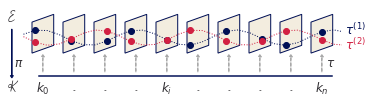
\includegraphics[width=1\linewidth]{figures/math/fiberbundle.png}
        \label{fig:data_sections}
    \end{figure}
    \begin{itemize}
        \item \dfiber\ is $\reals\times\reals$
        \item \dbase\ is interval $\left[0,1\right]$
        \item $\dsection^{(1)}$ is a $sin$ function
        \item $\dsection^{(2)}$ is a $cos$ function
        \item $\dsection^{(1)}, \dsection^{(2)} \in \Gamma(\dtotal)$
    \end{itemize}
  
\end{frame}

\begin{frame}{Sheafs}
    Restriction maps of a sheaf describe how local $\iota^*\dsection$ can be glued into larger sections \cite{ghristElementaryAppliedTopology2014,ghristHomologicalAlgebraData2018}.
    
    \begin{equation}
        \label{eq:sheaf}
        \begin{tikzcd}[ampersand replacement=\&]
            \iota^*\dtotal \arrow[d, "\pi"'] \arrow[r, "\iota^*", hook]             \& \dtotal \arrow[d, "\pi"']                  \\
            U \arrow[r, "\iota", hook] \arrow[u, "\iota^{*}\dsection"', bend right] \& \dbase \arrow[u, "\dsection"', bend right]
        \end{tikzcd}
    \end{equation}
    The inclusion map $\iota: U \rightarrow \dbase$ pulls \dtotal\ over $U$ such that the pulled back $\iota^*\dsection$ only contains records over $U \subset \dbase$.
\end{frame}

\subsection{Graphics}
\begin{frame}{Graphic Bundle}
    The graphics bundle is a tuple $(\gtotal,\,\gbase,\,\pi ,\,\gfiber)$ defined by the projection map $\pi$
    \begin{equation}
        \begin{tikzcd}[ampersand replacement=\&]
            \gfiber \arrow[r, hook] \& \gtotal \arrow[d, "\pi"'] \\
                              \& \gbase \arrow[u, "\gsection"', bend right]
        \end{tikzcd}
    \end{equation}
    where \gsection\ is the fully encoded graphic. 
    \pause
    \begin{block}{Example: 2D opaque image}
    The target display is $\gfiber=\reals^5$ with elements 
    \begin{equation*}
    (x,\, y,\, r,\, g,\, b) \in \gfiber
    \end{equation*}
    returned by \gsection\ such that a graphic has color and 2D position.
    \end{block}

\end{frame}
\begin{frame}{Graphic Continuity}
    The surjective map $\vindex: \gbase \rightarrow \dbase$
    \begin{equation}
        \begin{tikzcd}[ampersand replacement=\&]
            \dtotal \arrow[d, "\pi"'] \& \gtotal \arrow[d, "\pi"'] \\
            \dbase                   \& \gbase \arrow[l, "\vindex"']
        \end{tikzcd}
    \end{equation}
    goes from region $\gbasepoint \in \gbase_{\dbasepoint}$ to its associated point $\dbasepoint$ in data space. 
\pause
    \begin{figure}[H]
        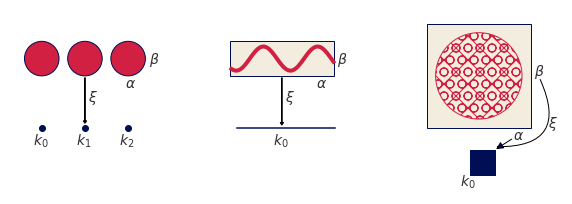
\includegraphics[width=1\textwidth]{figures/math/retraction_maps.png}
        \label{fig:graphic_retraction_map}
    \end{figure}
\end{frame}

\subsection{Artist}
\begin{frame}{Topological Equivariant Artist Model}
The topological artist \vartist\ is a monoid equivariant sheaf map 
\begin{equation}
    \label{eq:artist_diagram}
    \begin{tikzcd}[ampersand replacement=\&]
        \dtotal^{\prime} \arrow[r, "\vchannel"] \arrow[rd, "\pi"'] \& \vtotal \arrow[d, "\pi"] \& \vindex^*\vtotal \arrow[r, "\vmark"] \arrow[d, "\vindex^*\pi"'] \arrow[l, "\vindex^*"'] \& \gtotal \arrow[ld, "\pi"] \\
                                              \& \dbase                  \& \gbase \arrow[l, "\vindex"']                                              \&                    
        \end{tikzcd}
\end{equation}

where the artist $\vartist: \mathcal{O}(\dtotal) \rightarrow \mathcal{O}(\gtotal)$ takes as input $\dtotal^{\prime}=\mathcal{J}^{2}(\dtotal)$. 
\end{frame}

\begin{frame}{Visual Bundle}
    The visual bundle is a tuple $(\vtotal,\,\dbase,\,\pi ,\,\vfiber)$ defined by the projection map $\pi$
    \begin{equation}
        \begin{tikzcd}[ampersand replacement=\&]
            \vfiber \arrow[r, hook] \& \vtotal \arrow[d, "\pi"'] \\
                              \& \dbase \arrow[u, "\vsection"', bend right]
        \end{tikzcd}
    \end{equation}
    where \vsection\ is the visual variable encoding\cite{bertinIIPropertiesGraphic2011} of the data section \dsection. 
    \begin{block}{Example: position and color}
        Given an artist with parameters $\{xpos, ypos, color\}$, a sample visual section \vsection\ could be $\{.5, .5, (255, 20,147)\}$
    \end{block}
\end{frame}

\begin{frame}{Visual Channel Encoders}
We define the visual transformers \vchannel\ on components of the data bundle $\dsection_{i}$
\begin{equation}
    \label{eq:nu_expanded}
    \{\vchannel_{0}, \ldots, \vchannel_{n}\}: \{\dsection_{0}, \ldots, \dsection_{n}\} \mapsto \{\vsection_{0}, \ldots, \vsection_{n}\}
\end{equation}
as the set of equivariant maps with the constraint 
\begin{equation}
    \vchannel_i(m_{\delement}(\dtotal_i)) = \varphi(m_{\delement})(\vchannel_i(\dtotal_i))
\end{equation} 
where $\varphi:\monoid\rightarrow \monoid^{\prime}$ carries a homomorphism of monoid actions. 
\end{frame}

\begin{frame}{Example: Partial Order Equivariance}
    \begin{figure}
        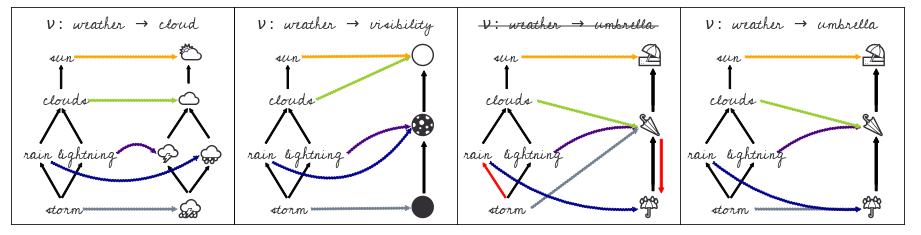
\includegraphics[width=1\textwidth]{figures/math/monoid_equivariant.png}
    \end{figure}
\end{frame}
\begin{frame}{Measurement Scale Groups}

\begin{table}[H]
    \begin{tabulary}{\textwidth}{llL}
        nominal & permutation &  $\text{if } \delement_1 \neq \delement_2 \text{ then } \vchannel (\delement_1) \neq\vchannel(\delement_2)$\\
        ordinal &  monotonic & $\text{if } \delement_1 \leq \delement_2 \text{ then } \vchannel (\delement_1) \leq \vchannel(\delement_2)$\\
        interval &  translation &  $\vchannel (x + c) = \vchannel(x) + c$ \\
        ratio &  scaling &  $\vchannel(xc) = \vchannel(x)*c $
    \end{tabulary}
\end{table}

    \pause
    \begin{block}{Invalid \vchannel}
     Given $\vchannel_{i}(x) = .5$ and $t(x) = x+2$,
    \pause    
    \begin{align*}
            \vchannel(t(\delement + 2)) & \overset{?}{=} \vchannel(\delement) + 2\\
            .5 &\neq .5 + 2
    \end{align*}
    \end{block}
\end{frame}

\begin{frame}{Visualization Assembly Function}
    \begin{figure}
        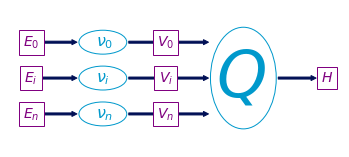
\includegraphics[width=\textwidth]{figures/math/path_of_q.png}
    \end{figure}
\end{frame}

\begin{frame}{Glyph}
    The glyph is the graphic generated by $\vmark(\gbase_{\dbasepathpoint})$ where the path connected components $\dbasepath \subset \dbase$ are defined 
    \begin{equation}
    \dbasepath = \{\dbasepathpoint \in \dbase \text{ s. t. } \exists \gamma \text{ s.t. } \gamma(0)=\dbasepoint \text{ and }\gamma(1)=\dbasepathpoint\}
    \end{equation}
    such that the  path $\gamma$ from \dbasepoint\ to \dbasepathpoint\ is a continuous function from the interval [0,1] and $\gbase_{\dbasepathpoint}$ is the region
    \begin{equation}
        \begin{tikzcd}[ampersand replacement=\&]
            \gtotal \arrow[r, shift left] \& \gbase_\dbasepathpoint \arrow[rr, "\vindex(\gbasepoint)", shift left] \arrow[l, "\gsection(\gbase_\dbasepathpoint)"] \& \& \dbasepath_{\dbasepoint} \arrow[ll, "\vindex^{-1}(\dbasepath)"]
            \end{tikzcd}
        \label{eq:mark}
    \end{equation}
    such that the glyph is differentiable, in keeping with Ziemkiewicz and Kosara's description of a glyph\cite{ziemkiewiczEmbeddingInformationVisualization2009}.
\end{frame}

\begin{frame}{Visualization Equivariance}
    If \vmark\ is applied to $\vsection, \vsection^{\prime}$ that generate the same \gsection\, 
    \begin{equation}
    \vmark(\vsection) = \vmark(\vsection^{\prime})\implies \vmark(m\circ\vsection) = \vmark(m\circ\vsection^{\prime})
    \end{equation}
    then the output of both sections acted on by the same monoid $m$ must be the same. 
    \pause
    \begin{figure}[H]
        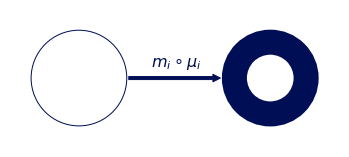
\includegraphics[width=\textwidth]{figures/math/diff_type_q.png}
    \end{figure}
\end{frame}

\begin{frame}{Scatter: $\vmark(xpos, ypos)(\alpha, \beta)$}
    \begin{figure}[H]
        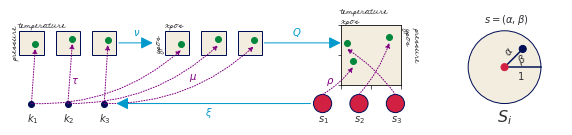
\includegraphics[width=1\textwidth]{figures/math/scatter.png}
    \end{figure}
    
    \begin{align*}
        x &= size *\alpha \cos(\beta) + xpos \\
        y &= size *\alpha \sin(\beta) + ypos
    \end{align*}    
\end{frame}

\begin{frame}{Line: $\vmark(xpos, \hat{n_{1}}, ypos, \hat{n_{2}})(\alpha, \beta)$ }
    \begin{figure}[H]
        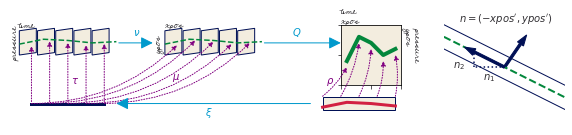
\includegraphics[width=1\textwidth]{figures/math/line.png}
    \end{figure}
        \begin{equation*}
            \lvert n \rvert = \sqrt{{n_{1}}^2 + {n_{2}}^2},\; 
            \hat{n_{1}} = \frac{n_1}{\lvert n \rvert}, \; \hat{n_{2}} = \frac{n_2}{\lvert n \rvert}
        \end{equation*}
    \begin{align*}
     x = xpos(\vindex(\alpha)) &+ width*\beta\hat{n_1}(\vindex(\alpha)) \\
     y = ypos(\vindex(\alpha)) &+ width*\beta\hat{n_2}(\vindex(\alpha)) 
    \end{align*}
\end{frame}

\begin{frame}{Image $\vmark(xpos, ypos, color)$}
    \begin{figure}[H]
        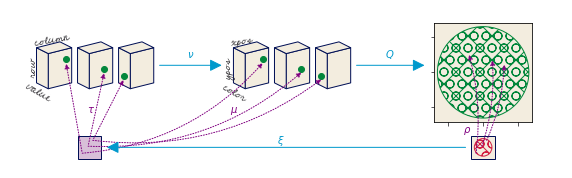
\includegraphics[width=1\textwidth]{figures/math/image.png}
    \end{figure}
    \begin{align*}
        R &= R(\vindex(\alpha, \beta))\\
        G &= G(\vindex(\alpha, \beta))\\
        B &= B(\vindex(\alpha, \beta))
    \end{align*}
\end{frame}

\begin{frame}{Assembly Function Factory}
\begin{figure}[H]
    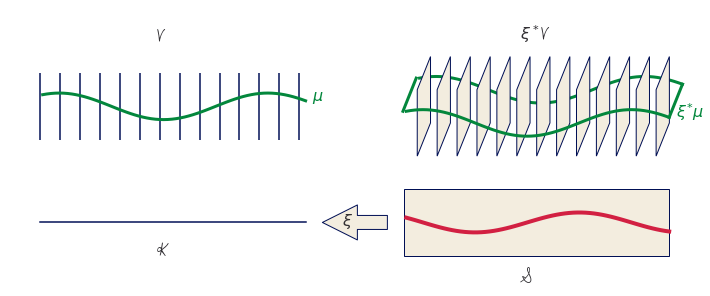
\includegraphics[width=1\textwidth]{figures/math/q_hat.png}
\end{figure}
\begin{equation}\label{eq:qhat_q_s}
    \vmarkd(\vsection(\dbasepoint))(\gbasepoint) \coloneqq \vmark((\vsectionpull)(\gbasepoint))
\end{equation} 
such \gbasepoint\ can be factored out when $\vpreimg = \gbasepoint$
\end{frame}

\begin{frame}{Composition of artists}
    Given the family of artists $(\dtotal_i: i\in I)$ on the same image
    \begin{equation}
        + \coloneqq \underset{i\in I}{\sqcup} \dtotal_{i}
    \end{equation}
    the + operator defines a simple composition of artists. 

    When artists share a base space 
    \begin{equation}
        \dbase_2 \hookrightarrow \dbase_1
    \end{equation}
    a composition operator can be defined such that the the artists can be considered to be acting on different components of the same section. 
\end{frame}

\begin{frame}{Equivalance class of artists}
    An approximation of the equivalence class of artists $\vartist^{\prime}$
    \begin{equation}
    \vartist \in \vartist^{\prime}: \vartist_{1} \equiv \vartist_{2}
    \end{equation}
    roughly treats two artists as equivalent if they 
    \begin{itemize}
        \item act on the same visual bundle \vtotal
        \item have the same assembly function \vmark 
        \item have the same continuity map \vindex 
    \end{itemize}
\end{frame}


\section{Prototype}
\subsection{Artist}
\begin{frame}[fragile]{Artist}
    \begin{minted}{python}
        class ArtistClass(matplotlib.artist.Artist):
            def __init__(self, data, transforms, *args, **kwargs):
                # properties that are specific to the graphic
                self.data = data 
                self.transforms = transforms
                super().__init__(*args, **kwargs)
        
            def assemble(self, **args):
                # set the properties of the graphic
        
            def draw(self, renderer):
                # returns K, indexed on fiber then key 
                view = self.data.view(self.axes) 
                # visual channel encoding applied fiberwise 
                visual = {p: t['encoder'](view[t['name']])
                          for p, t in self.transforms.items()}
                self.assemble(**visual)
                # pass configurations off to the renderer
                super().draw(renderer)
        \end{minted}
\end{frame}

\begin{frame}[fragile]{Artists: Scatter \& Line}
\begin{figure}[H]
    \begin{subfigure}{0.49\textwidth}
        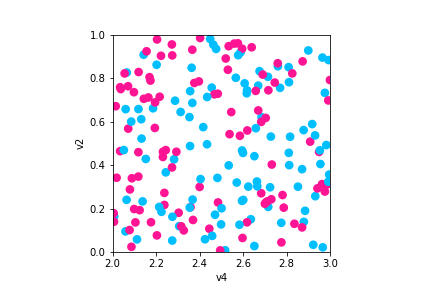
\includegraphics[width=\textwidth]{figures/code/scatter_0.png}
    \end{subfigure}
    \begin{subfigure}{0.49\textwidth}
        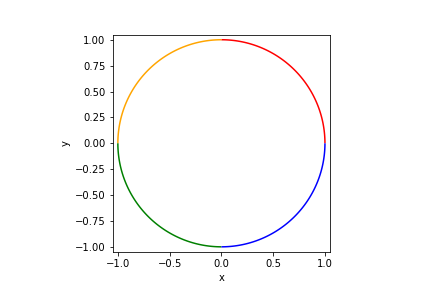
\includegraphics[width=\textwidth]{figures/code/line_1.png}
    \end{subfigure}
\end{figure}
\begin{columns}
\column{0.49\textwidth}
\begin{minted}{python}
fig, ax = plt.subplots()
artist = Point(data, transforms)
ax.add_artist(artist)
\end{minted}
\column{.49\textwidth}
\begin{minted}{python}
fig, ax = plt.subplots()
artist = Line(data, transforms)
ax.add_artist(artist)
\end{minted}
\end{columns}
\end{frame}

\begin{frame}[fragile]{Artists: Scatter \& Line}
\begin{minted}{python}
class Point(mcollections.Collection):
    def assemble(self, x, y, s, facecolors='C0' ):
        # construct geometries of the circle glyphs in visual coordinates
        self._paths = [mpath.Path.circle(center=(xi,yi), radius=si) 
                    for (xi, yi, si) in zip(x, y, s)] 
        # set attributes of glyphs, these are vectorized 
        # circles and facecolors are lists of the same size
        self.set_facecolors(facecolors)
\end{minted} 
    \pause
\begin{minted}{python}
class Line(mcollections.LineCollection):
    def assemble(self, x, y, color='C0'):
        #assemble line marks as set of segments 
        segments = [np.vstack((vx, vy)).T for vx, vy in zip(x, y)]
        self.set_segments(segments)
        self.set_color(color)
\end{minted}
\end{frame}

\begin{frame}[fragile]{Visual Transformations}
\begin{minted}{python}
cmap =  color.Categorical({'true':'deeppink', 'false':'deepskyblue'})
transforms = {'x': {'name': 'v4', 'encoder': lambda x: x},
                'y': {'name': 'v2', 'encoder': lambda x: x},
                'facecolors': {'name':'v3', 'encoder': cmap}, 
                's':{'name': None , 
                    'encoder': lambda _: itertools.repeat(.02)}}
\end{minted}
    \begin{itemize}
        \item \mintinline{python}{lambda x: x} is identity \vchannel\
        \item \mintinline{python}|{'name':None}| map into \vfiber\ without corresponding \dsection\
        \item \mintinline{python}{color.Categorical} is custom \vchannel
    \end{itemize}
\end{frame}

\begin{frame}[fragile]{Custom Complex \vchannel}
\begin{minted}{python}
class Categorical:
    def __init__(self, mapping):
        # check that the conversion is to valid colors
        assert(mcolors.is_color_like(color) for color in mapping.values())
        self._mapping = mapping

    def __call__(self, value):
        # convert value to a color
        return [mcolors.to_rgba(self._mapping[v]) for v in values]
\end{minted}
\pause
That we can test for action equivariance
\begin{minted}{python}
def test_nominal(values, encoder):
    m1 = list(zip(values, encoder(values)))
    random.shuffle(values)
    m2 = list(zip(values, encoder(values)))
    assert sorted(m1) == sorted(m2)
\end{minted}
\end{frame}
\subsection{Data}
\begin{frame}[fragile]{Fiber Bundle}
\begin{minted}{python}
@dataclass
class FiberBundle:
"""
Attributes
----------
K: {'tables': []}
F: {variable name: type}
"""
    K: dict 
    F: dict
\end{minted}
\end{frame}

\begin{frame}[fragile]{Discrete Connectivity}
\begin{minted}{python}
class VertexSimplex: #maybe change name to something else
    """Fiberbundle is consistent across all sections
    """
    FB = FiberBundle({'tables': ['vertex']},  
            {'v1': float, 'v2': str, 'v3': float})

    def __init__(self, sid = 45, size=1000, max_key=10**10):
        # create random list of keys
    def tau(self, k):
        # e1 is sampled from F1, e2 from F2, etc...
        return (k, (e1, e2, e3, e4))
\end{minted}
\end{frame}

\begin{frame}[fragile]{1D Continuous Connectivity}
\begin{minted}{python}
class EdgeSimplex: 
    FB = FiberBundle({'tables': ['vertex','edge']},
                         {'x' : float, 'y':  float, 
                         'color':mtypes.Color()}})
    def __init__(self, num_edges=4, num_samples=1000): 
        self.keys = range(num_edge) #edge id
        self.distances = np.linspace(0,1, num_samples)
        # half generlized representation of arcs on a circle
        self.angle_samples = np.linspace(0, 2*np.pi, len(self.keys)+1)
    @staticmethod
    def _color(edge):
        return ['red','orange', 'green','blue'][edge%4]
    @staticmethod
    def _xy(edge, distances, start=0, end=2*np.pi):
        # start and end are parameterizations b/c really there is 
        angles = (distances *(end-start)) + start
        return np.cos(angles), np.sin(angles)
    def tau(self, k): #will fix location on page on revision
        x, y = self._xy(k, self.distances, 
                        self.angle_samples[k], self.angle_samples[k+1]) 
        color = self._color(k) 
        return (k, (x, y, color))
\end{minted}
\end{frame}

\begin{frame}[fragile]{View}
\begin{minted}{python}
def view(self, axes):
    table = defaultdict(list)
    for k in self.keys:
        table['index'].append(k)
        for (name, value) in zip(self.FB.fiber.keys(), self.tau(k)[1]):
            table[name].append(value)
    return table
\end{minted}
\begin{description}
    \item [\mintinline{python}{VertexSimplex}] (name, value), value is scaler
    \item [\mintinline{python}{EdgeSimplex}]  (name, value), value is [x0, ..., xn]
\end{description}
\end{frame}
\begin{frame}[fragile]{Same Artist, Different Data Configurations}
    \begin{figure}[H]
        \begin{subfigure}{0.49\textwidth}
            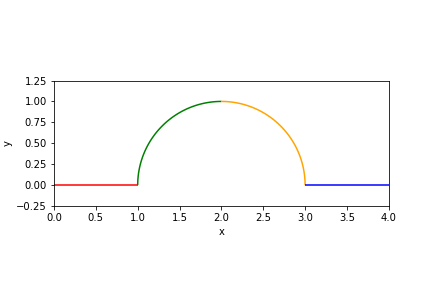
\includegraphics[width=\textwidth]{figures/code/linec_1.png}
        \end{subfigure}
        \begin{subfigure}{0.49\textwidth}
            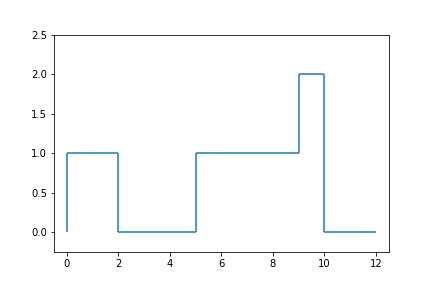
\includegraphics[width=\textwidth]{figures/code/lined_1.png}
        \end{subfigure}
    \end{figure}
\begin{minted}{Python}
simplex.GraphLine(FB, edge_table, vertex_table, 
                      connect=True)
simplex.GraphLine(FB, edge_table, vertex_table, 
                      num_samples=2, connect=False)
\end{minted}
\end{frame}

\section{Conclusion}
\begin{frame}{Summary}
    \begin{itemize}
        \item structure preserving maps from data to visual representation:
            \begin{itemize}
                \item data and graphics have equivalent continuity
                \item properties are equivariant under monoid actions
            \end{itemize}  
        \item fiber bundles with a schema are structure rich abstractions of 
            \begin{itemize}
                \item topologically complex heterogenous data 
                \item target display spaces
            \end{itemize}
        \item model can be iteratively integrated into existing Matplotlib architecture
    \end{itemize}
\end{frame}

\begin{frame}{Proposed Dissertation}
\begin{itemize}
    \item expansion of the mathematical framework to include worked out simple and complex addition
    \item formalization of definition of equivalance class \vartisteq
    \item implementation of artist with explicit \vindex\
    \item specification of interactive visualization
    \item mathematical formulation of a graphic with axes labeling
    \item implementation of new prototype artists that do not inherit from Matplotlib artists
    \item provisional mathematics and implementation of user level composite artists
    \item proof of concept domain specific user facing library 
\end{itemize}
\end{frame}

\section{References}
\begin{frame}[allowframebreaks]{References}
\printbibliography
\end{frame}
\appendix 
\begin{frame}{Rendering: Define a Pixel}
    \begin{columns}
        \column{0.5\textwidth}
        Given a pixel
        \begin{equation}
        p=\left[y_{top}, y_{bottom}, x_{right}, x_{left}\right]
        \end{equation}
        the inverse map of the bounding box 
        \begin{equation}
        \gbase_{p} ={\gsection_{xy}}^{-1}(p)
        \end{equation}
        is a region $\gbase_p \subset \gbase$ such that 
        \begin{align}
            \scriptstyle r_p &= \scriptstyle \iint\limits_{S_p} \rho_r(s)ds^{2}\\
            \scriptstyle g_p &= \scriptstyle \iint\limits_{S_p} \rho_g(s)ds^{2}\\
            \scriptstyle  b_p &= \scriptstyle \iint\limits_{S_p} \rho_b(s)ds^{2}
        \end{align}
        yields the color of the pixel. 
        \column{0.5\textwidth}
        \begin{figure}[H]
            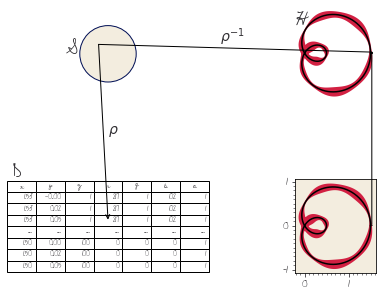
\includegraphics[width=\textwidth]{figures/math/render.png}
        \end{figure}
    \end{columns}
\end{frame}
\begin{frame}{\vfiber\ Components}
    
\begin{table}[H]
    \renewcommand{\arraystretch}{2}
    \begin{tabulary}{\textwidth}{|l|L|l|}\hline
     $\bm{\vchannel_{i}}$                      & $\bm{\vsection_{i}}$                                                            & $\bm{codomain(\vchannel_{i}) \subset \vfiber_{i}}$  \\ \hline                                              
    position                    & x, y, z, theta, r                                                          & $\mathbb{R}$   \\ \hline
    size                        & linewidth, markersize                                            & $\mathbb{R}^{+}$   \\ \hline
    shape                       & markerstyle                                                      & $\{f_{0}, \ldots, f_{n}\}$ \\ \hline
    color                       & color, facecolor, markerfacecolor, edgecolor  & $\mathbb{R}^{4}$ \\ \hline
    \multirow{2}{*}{texture}    & hatch                                                            & $\mathbb{N}^{10}$\\\cline{2-3}
                                & linestyle                                                        & $(\mathbb{R}, \mathbb{R^+}^{n, n\%2=0})$ \\ \hline              
    \end{tabulary}
    \label{tab:mpl_visual_variable_fiber}
\end{table}
\end{frame}
\begin{frame}[fragile]{GraphLine Data Model}
\begin{minted}{python}
class GraphLine:
    def __init__(self, FB, edge_table, vertex_table, num_samples=1000,
                        connect=False):
        #set args as attributes and generate distance
        if connect: # test connectivity if edges are continuous
            assert edge_table.keys() == self.FB.F.keys()
            assert is_continuous(vertex_table)

    def tau(self, k):
        # evaluates functions defined in edge table
        return(k, (self.edges[c][k](self.distances) 
                        for c in self.FB.F.keys()))

    def view(self, axes):
        # walk the edge_vertex table to return the edge function
        table = defaultdict(list)
        for (i, (start, end)) in sorted(zip(self.ids, self.vertices), 
                                            key=lambda v:v[1][0]):
            table['index'].append(i)
            # same as view for line, returns nested list
            for (name, value) in zip(self.FB.F.keys(), self.tau(i)[1]):
                table[name].append(value)
        return table
\end{minted}
\end{frame}

\end{document}

